\documentclass{article}

% NeurIPS 2026 style
\usepackage[final,main]{neurips_2026}

% Core packages
\usepackage[utf8]{inputenc}
\usepackage[T1]{fontenc}
\usepackage{hyperref}
\usepackage{url}
\usepackage{booktabs}
\usepackage{amsfonts}
\usepackage{amsmath}
\usepackage{amssymb}
\usepackage{amsthm}
\usepackage{nicefrac}
\usepackage{microtype}
\usepackage{xcolor}
\usepackage{graphicx}
% Algorithm packages not available, using custom environment
% Simple algorithm environment replacement
\newcounter{algorithm}
\newenvironment{algorithm}[1][t]{%
  \refstepcounter{algorithm}%
  \begin{center}%
  \begin{minipage}{0.95\textwidth}%
  \hrule
  \vspace{0.5em}%
  \textbf{Algorithm \thealgorithm:}%
}{%
  \vspace{0.5em}%
  \hrule
  \end{minipage}%
  \end{center}%
}

\newcommand{\algcaption}[1]{\textbf{#1}\par\vspace{0.3em}}

% Algorithmic commands
\newcommand{\REQUIRE}{\textbf{Require:} }
\newcommand{\ENSURE}{\textbf{Ensure:} }
\newcommand{\STATE}{\par\hspace{1em}}
\newcommand{\IF}{\textbf{if} }
\newcommand{\THEN}{\textbf{then}}
\newcommand{\ELSE}{\par\hspace{1em}\textbf{else}}
\newcommand{\ENDIF}{\par\hspace{1em}\textbf{end if}}
\newcommand{\FOR}{\textbf{for} }
\newcommand{\ENDFOR}{\par\hspace{1em}\textbf{end for}}
\newcommand{\RETURN}{\textbf{return} }

\newenvironment{algorithmic}[1][1]{%
  \small
  \begin{flushleft}%
}{%
  \end{flushleft}%
}

\usepackage{multirow}
\usepackage{subcaption}
\usepackage{cleveref}
\usepackage{tikz}
\usetikzlibrary{positioning}
\setcitestyle{numbers,square,comma,sort&compress}

% Title and authors
\title{EVICT: Evidence-Conditioned Investigation with Calibrated Triage for Static Analysis Alerts}

\author{%
  Anonymous Authors\\
  Anonymous Institution\\
  \texttt{anonymous@institution.edu}
}

\begin{document}

\maketitle

\begin{abstract}
Static analysis tools are routinely disabled or ignored in practice because false-positive (FP) rates of 40--90\%~\cite{johnson2013,christakis2016} and 10--20 minutes of triage time per alert~\cite{tencent2023} render exhaustive review intractable. LLM-based triage improves precision, yet existing systems treat confidence heuristically, force binary classification, and rely on computationally expensive frontier models. We present \textbf{EVICT} (Evidence-Conditioned Investigation with Calibrated Triage), which reframes alert triage as a \emph{cost-sensitive selective prediction} problem: the system accepts only those alerts for which calibrated evidence supports a reliable decision, and explicitly defers uncertain cases to human review. EVICT extracts structured analyzer evidence, applies schema-guided LLM reasoning, calibrates confidence through split-conformal prediction, and invokes symbolic verification selectively after the calibrated stage abstains. This sequencing lets us state finite-sample validity for the \emph{pre-escalation} selective predictor while treating symbolic checks as a targeted audit mechanism outside the conformal guarantee.

We contribute two complementary empirical studies. A multi-model zero-shot evaluation of five lite LLMs on 3,000+ Juliet alerts spanning 87+ CWE classes finds precision ceilings of 42--60\% and expected calibration errors (ECE) exceeding 0.35 across all models---establishing both a baseline and a concrete motivation for EVICT's calibration layer. Among the models evaluated, Claude Haiku 4.5 achieves the highest precision (59.9\%) and FP mitigation rate (80.3\%), while GPT-4o Mini achieves the highest recall (90.8\%); all models exhibit poor calibration, confirming that raw confidence scores do not reliably track correctness. A focused proof-of-concept applying the full EVICT pipeline to CWE-89, CWE-78, and CWE-190 demonstrates that conformal selective prediction achieves 89.3\% precision at 87.3\% coverage with ECE\,=\,0.08---improving over an evidence-free baseline (83.5\% precision, ECE\,=\,0.15) and reducing selective risk from 0.165 to 0.107. Symbolic escalation further lifts precision to 91.2\% at 89.6\% coverage, correcting 23 LLM errors of which 73.9\% were safety-critical FP\,$\to$\,TP reversals. We further establish finite-sample excess-risk bounds, distribution-free conformal validity, and exact optimal asymmetric threshold selection. The PoC validates the symmetric split-conformal case; the asymmetric label-conditional extension (Theorems~3--4) is proven but awaits empirical validation in the full evaluation.
\end{abstract}

% Main sections
\section{Introduction}
\label{sec:introduction}

Static analysis tools are routinely deployed in secure software engineering pipelines precisely because they are scalable and conservative: they sacrifice specificity for recall, flagging every potential vulnerability that cannot be ruled out by over-approximate reasoning. In industrial practice, this conservatism produces false-positive (FP) rates between 40\% and 90\%~\cite{johnson2013,christakis2016}, with manual triage requiring 10--20 minutes per alert~\cite{tencent2023}. At enterprise scale, the cumulative review burden is a material engineering cost that limits the practical impact of static analysis.

Recent work demonstrates that large language models (LLMs) can reduce this burden by conditioning on structured analyzer evidence---code slices, data-flow traces, and path constraints---to distinguish real vulnerabilities from analysis artifacts~\cite{llm4fpm2024,llm4pfa2024,buglens2024,adataint2023}. However, two deployment barriers persist. The closest prior system, IRIS~\cite{li2025iris}, uses LLM-assisted specification inference to validate CodeQL findings but requires generating per-vulnerability formal specifications and relies on frontier-model reasoning without principled abstention. First, state-of-the-art triage systems rely on computationally expensive frontier models; replacing them with fast, cost-effective ``lite'' models (e.g., Gemini Flash Lite, Claude Haiku, GPT nano) reveals a calibration collapse: our multi-model evaluation on 3,000+ Juliet alerts spanning 87 CWE classes finds zero-shot precision ceilings of 42--60\% and expected calibration errors (ECE) exceeding 0.35, confirming that raw model confidence does not reliably track correctness in the lite-model regime. Second, existing LLM triage systems force binary classification without formalizing \emph{abstention} as a first-class action with auditable guarantees---an omission that is unsafe when missed vulnerabilities carry asymmetric costs.

We address both barriers with \textbf{EVICT} (Evidence-Conditioned Investigation with Calibrated Triage). EVICT casts alert triage as a \emph{cost-sensitive selective prediction} problem~\cite{elyaniv2010,geifman2017}: the system learns both a predictor $h$ and a rejector $g$, where $g(x) = 0$ explicitly defers uncertain alerts to human review, and $g(x) = 1$ accepts only those for which calibrated evidence supports a reliable decision. This framing converts the accept/abstain threshold from an arbitrary hyperparameter into the solution of a finite-sample optimization problem, ties automation to formal risk control, and creates a principled trigger for targeted symbolic verification.

\paragraph{Contributions.}

\textbf{(1) Formalization.} We cast alert triage as a cost-sensitive selective prediction problem with asymmetric costs, derive a finite-sample excess-risk bound for threshold selection with label-specific convergence rates (Theorem~\ref{thm:risk}), and prove distribution-free conformal validity for the pre-escalation selective predictor (Theorem~\ref{thm:conformal}). A label-conditional extension with exact threshold optimization under asymmetric costs is established in Theorems~\ref{thm:label_conditional} and~\ref{thm:exact_opt}.

\textbf{(2) Evidence-conditioned reasoning with calibrated confidence.} EVICT extracts a structured EvidencePack (code slice, data-flow summary, path constraints) from SARIF-format analyzer output and prompts a lite LLM with a fixed four-step reasoning schema. Confidence is estimated via logit margins or self-consistency vote shares ($k = 5$), then calibrated using \textbf{Split-Conformal Prediction} (\textbf{Algorithm~\ref{alg:conformal}}). An alert is accepted as TP or FP only when the conformal prediction set is a singleton; otherwise the system abstains.

\textbf{(3) Conditional neuro-symbolic escalation.} When the calibrated stage abstains, EVICT invokes a symbolic escalator---\textbf{Java PathFinder (JPF)} for Java---on deferred alerts. Symbolic \texttt{UNKNOWN} results and timeouts (8.1\% empirical rate) are strictly treated as continued abstentions rather than forced classifications, preserving the safety semantics of the pre-escalation stage.

\paragraph{Empirical contributions.} We contribute three complementary empirical studies. A \emph{multi-model zero-shot baseline study} evaluates five lite LLMs across 87+ CWE classes, finding precision ceilings of 42--60\% and ECE $> 0.35$ throughout. A \emph{multi-model conformal calibration study} applies the full EVICT pipeline to six models spanning three training paradigms (reasoning, instruction-tuned, code-specialized) on CWE-89/78/190 with $k=5$ self-consistency sampling and 5-fold cross-validation. This study reveals a previously unreported finding: \textbf{the quality of the self-consistency confidence signal depends more on the model's training objective than on model size}. Reasoning models (R1-Distill-14B) produce diverse vote-share (36\% unanimous, ECE 0.335), while instruction-tuned and code-specialized models produce degenerate confidence (85--98\% unanimous, ECE 0.51--0.62), making conformal calibration effective only for the former. A \emph{real-world validation} on CWE-Bench-Java (549 CodeQL alerts, 45 projects) confirms the TP-bias pattern and reveals a code-specialization paradox: code models achieve the best FP rejection (TN=184) despite the worst confidence quality. We further project that frontier reasoning models (GPT-4.5, Claude Sonnet 4) will be the first model class where conformal calibration produces practically significant precision gains ($+3$--$10$pp).

Section~\ref{sec:background} surveys related work. Sections~\ref{sec:methodology} and~\ref{sec:theory} specify the method and its formal guarantees. Section~\ref{sec:preliminary} reports the two empirical studies. The remaining sections describe the planned full evaluation, discuss limitations, and address broader impact.

\section{Background and Related Work}
\label{sec:background}

\subsection{Static Analysis and False Positives}

Static analyzers (e.g., SpotBugs, Infer, CodeQL) are deliberately sound-over-complete: they prioritize recall, yielding FP rates of 40--90\% in industrial deployments~\cite{johnson2013,christakis2016}. Because manual triage costs 10--20 minutes per alert~\cite{tencent2023}, organizations are frequently forced to choose between alert fatigue and reduced analyzer coverage. Any automated triage system must therefore be judged not only by precision on the accepted set, but by whether it reduces the review burden while keeping the false-negative rate on auto-dismissed alerts acceptably low.

\subsection{LLM-Based Alert Triage}

Recent systems exploit structured analyzer evidence---slices, call chains, data-flow paths---to condition LLM classification, demonstrating that grounding LLM reasoning in code-level evidence materially improves precision over ungrounded prompting~\cite{llm4fpm2024,llm4pfa2024,buglens2024,adataint2023}. However, these systems uniformly frame triage as forced binary classification, rely on computationally expensive frontier models, and treat model confidence as an opaque score rather than a calibrated probability. As a result, they cannot provide coverage or risk guarantees, and they offer no principled mechanism for deferral.

EVICT differs along two axes: it targets the cost-effective lite-model regime, and it enforces safety through formalized abstention rather than relying on high raw accuracy. Our multi-model zero-shot baseline study (Table~\ref{tab:multimodel}) confirms that lite models achieve only 42--60\% precision with ECE $> 0.35$ without calibration---numbers that are unacceptable for production use and consistent with well-documented calibration pathologies of instruction-tuned LLMs~\cite{guo2024calibration,kadavath2022}.

\subsection{Selective Prediction and Calibration}

EVICT builds on the selective-prediction framework~\cite{elyaniv2010,geifman2017}, where a predictor proposes a label and a rejector decides whether to commit or defer. The key operational advantage of selective prediction over threshold-based filtering is that the reject decision is a first-class action with an associated cost, making risk--coverage tradeoffs explicit and auditable rather than implicit in a tuned threshold.

Calibration is essential because LLM confidence scores are systematically misaligned with correctness, especially under distribution shift~\cite{guo2024calibration,kadavath2022}. Unlike post-hoc temperature scaling~\cite{guo2017calibration} or Bayesian binning~\cite{naeini2015}, which improve calibration on average without distribution-free coverage guarantees, Split-Conformal Prediction~\cite{vovk2005,angelopoulos2021} provides exact finite-sample marginal coverage for any score function without distributional assumptions. This makes it well-suited to the code-analysis domain, where label distributions shift across projects and analyzers.

\subsection{Neuro-Symbolic Verification and Shift}

EVICT functions as a conditional neuro-symbolic verifier: the LLM handles semantic interpretation of analyzer evidence, while symbolic engines are reserved for cases where the calibrated LLM abstains or a high-severity dismissal warrants scrutiny. This conditional invocation transforms symbolic analysis from a universal computational bottleneck into a targeted audit mechanism.

The design choice of treating symbolic \texttt{UNKNOWN} results and timeouts as continued abstentions---rather than mapping them to a forced label---is a deliberate safety-preservation decision. Empirically, SMT UNKNOWN rates of 5--15\% are common on non-trivial program constraint systems~\cite{warp2023}, and 8.1\% of escalated alerts in our pilot dataset fell into this category. By treating UNKNOWN as an abstention signal consistent with the rejector $g(x) = 0$, EVICT avoids forcing a classification when both statistical evidence and symbolic verification fail, ensuring robustness under project and framework shift. The finite-sample conformal guarantee applies only to the pre-escalation selective predictor; symbolic verification operates as a separate, post-calibration audit layer whose outputs are reported independently.

\section{Approach}
\label{sec:methodology}

\subsection{Problem Formulation}

Each alert $x\in\mathcal{X}$ has a label $y\in\{\mathrm{TP},\mathrm{FP}\}$. EVICT learns a predictor $h:\mathcal{X}\rightarrow\{\mathrm{TP},\mathrm{FP}\}$ and a rejector $g:\mathcal{X}\rightarrow\{0,1\}$, where $g(x)=1$ commits to $h(x)$ and $g(x)=0$ abstains. Coverage is $\Pr[g(x)=1]$, i.e., the fraction of all alerts accepted before optional symbolic escalation.

The objective is the cost-sensitive selective risk
\begin{equation}
R(h,g)=\alpha_{\mathrm{cost}} R_{\mathrm{FN}}(h,g)+\beta_{\mathrm{cost}} R_{\mathrm{FP}}(h,g)+\gamma_{\mathrm{abs}} R_{\mathrm{abstain}}(g),
\end{equation}
with $\alpha_{\mathrm{cost}}>\beta_{\mathrm{cost}}$ in security settings. We reserve $\alpha_{\mathrm{TP}}$ and $\alpha_{\mathrm{FP}}$ for conformal miscoverage rates in Section~\ref{sec:theory}; this avoids overloading cost weights with conformal error probabilities. We write $k_{\mathrm{sc}}$ for the number of self-consistency samples per alert and $F$ for cross-validation folds.

\subsection{System Overview}

Figure~\ref{fig:architecture} summarizes the four-stage pipeline. The key sequencing rule is that conformal calibration produces the pre-escalation accept/abstain decision. Symbolic verification is a separate audit layer and never retroactively changes the coverage guarantee without recalibration.

\begin{figure}[t]
\centering
\resizebox{0.95\linewidth}{!}{%
\begin{tikzpicture}[
  node distance=0.55cm,
  box/.style={draw, rounded corners, align=center, font=\sffamily, text width=7.9cm, minimum height=0.85cm},
  side/.style={draw, rounded corners, align=center, font=\sffamily, text width=4.4cm, minimum height=0.85cm},
  arrow/.style={-{Stealth[length=2mm]}, thick},
  dashedarrow/.style={-{Stealth[length=2mm]}, thick, dashed}
]
\node[box, fill=blue!8] (a) {Static-analyzer alerts\\\small SARIF, rule, severity, source/sink locations};
\node[box, fill=green!8, below=of a] (b) {EvidencePack construction\\\small slice, data-flow summary, path constraints, incompleteness flags};
\node[box, fill=purple!8, below=of b] (c) {LLM verifier\\\small schema-guided or contrastive prompt; TP/FP/ABSTAIN rationale};
\node[box, fill=orange!10, below=of c] (d) {Conformal calibrator\\\small nonconformity score $A(x,y)$; singleton-reject prediction set};
\node[box, fill=yellow!15, below=of d] (e) {Pre-escalation decision\\\small singleton $\Rightarrow$ accept TP/FP; empty or multi-label $\Rightarrow$ abstain};
\node[side, fill=red!8, right=0.7cm of e] (f) {Conditional symbolic escalation\\\small Z3, JPF, KLEE; UNKNOWN/timeout $\Rightarrow$ abstain};
\node[box, fill=green!8, below=of e] (g) {Triaged alert with evidence-linked rationale};
\draw[arrow] (a) -- (b);
\draw[arrow] (b) -- (c);
\draw[arrow] (c) -- (d);
\draw[arrow] (d) -- (e);
\draw[arrow] (e) -- node[left, font=\scriptsize] {accepted} (g);
\draw[dashedarrow] (e) -- node[above, font=\scriptsize] {abstain/audit} (f);
\draw[arrow] (f) |- (g);
\end{tikzpicture}}
\Description{Pipeline diagram showing static-analysis alerts converted to EvidencePacks, checked by an LLM verifier, calibrated by conformal prediction, optionally escalated to symbolic verification, and emitted as triaged alerts.}
\caption{EVICT architecture. The conformal guarantee covers the pre-escalation singleton-reject decision. Symbolic escalation is a post-calibration audit layer.}
\label{fig:architecture}
\end{figure}

\subsection{Evidence Extraction}

The evidence extractor parses SARIF output~\cite{sarif2020} and constructs an \emph{EvidencePack}: alert metadata, source and sink locations, the analyzer-reported flow path when present, a bounded backward/forward program slice~\cite{weiser1984}, normalized branch/path constraints, and completeness flags. Java extraction uses JDT-style AST traversal; C/C++ extraction uses Clang-style parsing. Incomplete evidence is preserved explicitly through flags such as \texttt{flow\_partial} and \texttt{constraints\_missing}. These flags instruct the verifier to treat affected preconditions as ambiguous rather than hallucinating missing facts.

\subsection{Schema-Guided and Contrastive Verification}

The base verifier prompt follows four steps: restate the analyzer claim, enumerate the preconditions required for the alert to be real, check each precondition against the EvidencePack, and emit TP, FP, or ABSTAIN with confidence and rationale. The goal is not unconstrained chain-of-thought, but evidence-linked reasoning that a developer can audit.

The contrastive prompt is a first-class contribution. It changes the verifier from one-directional classification to adversarial evidence weighing: (1) construct the strongest TP argument, (2) construct the strongest FP argument, (3) explicitly inspect sanitizer, infeasible-path, and non-attacker-input evidence, and (4) weigh both sides before deciding. Study~4 shows that this intervention causes meaningful self-consistency disagreement without changing the model.

\subsection{Confidence and Conformal Calibration}

For logit-access models, EVICT uses normalized label probabilities over $\{\mathrm{TP},\mathrm{FP}\}$ and the nonconformity score
\begin{equation}
A(x,y)=1-p_\theta(y\mid x).
\end{equation}
For API-only models, EVICT samples $k_{\mathrm{sc}}=5$ completions at temperature 0.7 and uses vote share $v(y\mid x)$:
\begin{equation}
A(x,y)=1-v(y\mid x).
\end{equation}
Vote share and logit margin are preferred to entropy because the binary label space makes entropy too coarse to distinguish many operationally different TP/FP configurations.

Split-conformal calibration computes a threshold $\hat q$ on held-out calibration alerts. At inference time, EVICT forms
\begin{equation}
\hat C(x)=\{y\in\{\mathrm{TP},\mathrm{FP}\}: A(x,y)\le \hat q\}.
\end{equation}
If $|\hat C(x)|=1$, the system accepts the singleton label. If $\hat C(x)$ is empty or contains both labels, the system abstains. Algorithm~\ref{alg:conformal} gives the full procedure.

\subsection{Conditional Symbolic Escalation}

Abstained alerts may be escalated to symbolic tools: Z3 for path feasibility, Java PathFinder for Java, and KLEE for C/C++~\cite{jpf2003,spf2013,klee2008}. SAT or counterexample results support TP; UNSAT or exhaustive infeasibility supports FP. SMT \texttt{UNKNOWN}, tool timeouts, and missing constraints are treated strictly as continued abstentions. In the symbolic characterization study, the Z3 timeout is 2s, the JPF/KLEE timeout is 10s, and 15/184 symbolic invocations (8.1\%) return \texttt{UNKNOWN}; all are retained as abstentions.

\section{Theoretical Analysis}
\label{sec:theory}

\newtheorem{theorem}{Theorem}

All guarantees in this section concern the \emph{pre-escalation} selective predictor, i.e., the conformal accept/abstain stage before symbolic verification. They assume exchangeability between calibration and test alerts; the consequences of weakening this assumption under project shift are discussed at the end of the section. The current empirical section instantiates only the symmetric split-conformal special case; the asymmetric results below provide the decision-theoretic foundation that motivates the full evaluation rather than describing a procedure already validated by the pilot study. Full derivations appear in Appendix~\ref{app:proofs}.

\begin{theorem}[Cost-aware finite-sample excess risk]
\label{thm:risk}
Partition the calibration data into an independent grid-construction split $D^{(G)}$ and evaluation split $D^{(E)}$. Let $\mathcal Q_G$ be the finite set of feasible asymmetric TP/FP threshold pairs induced by $D^{(G)}$, let
\[
\hat q\in\arg\min_{q\in\mathcal Q_G}\hat R_E(q),
\qquad
q_G^\star\in\arg\min_{q\in\mathcal Q_G}R(q),
\]
and define $C_{\mathrm{TP}}=\max(\alpha,\gamma)$, $C_{\mathrm{FP}}=\max(\beta,\gamma)$. If $m^{(E)}_{\mathrm{TP}}$ and $m^{(E)}_{\mathrm{FP}}$ are the TP and FP counts in $D^{(E)}$, then, conditional on $D^{(G)}$, with probability at least $1-\delta$ over $D^{(E)}$,
\begin{equation}
R(\hat q)-R(q_G^\star)
\le
2\pi_{\mathrm{TP}} C_{\mathrm{TP}}
\sqrt{\frac{\log(4|\mathcal Q_G|/\delta)}{2m^{(E)}_{\mathrm{TP}}}}
+
2\pi_{\mathrm{FP}} C_{\mathrm{FP}}
\sqrt{\frac{\log(4|\mathcal Q_G|/\delta)}{2m^{(E)}_{\mathrm{FP}}}}.
\end{equation}
\end{theorem}

Theorem~\ref{thm:risk} gives the statistically appropriate guarantee for EVICT because it analyzes the finite threshold family that is actually selected on the calibration split. The excess-risk bound decomposes by label: generalization is controlled by the effective loss magnitude and sample size of each stratum, rather than a single pooled count. In asymmetric security regimes where $\alpha \gg \beta$, the TP term can dominate even when total sample size is large. The $1/\sqrt{m_y}$ dependence is tight up to constants (Appendix~\ref{app:proofs}).

\begin{theorem}[Conformal validity]
\label{thm:conformal}
If the calibration set and test alert are exchangeable, the conformal prediction set $\hat C(x)$ satisfies
\begin{equation}
\mathbb{P}[y\in \hat C(x)]\ge 1-\alpha
\end{equation}
for any score function.
\end{theorem}

EVICT converts this set-valued guarantee into a reject option by predicting only on singleton sets: a singleton gives a committed TP or FP label, while an empty or multi-label set triggers abstention. The singleton frequency is therefore the primary operational diagnostic for the calibrated automation stage.

\begin{theorem}[Label-conditional asymmetric conformal validity]
\label{thm:label_conditional}
Let $\hat q_{\mathrm{TP}}$ and $\hat q_{\mathrm{FP}}$ be label-specific conformal quantiles computed from the TP and FP calibration subsets with target miscoverage rates $\alpha_{\mathrm{TP}}$ and $\alpha_{\mathrm{FP}}$. Define
\[
\hat C_{\mathrm{asym}}(x)=\{y\in\{\mathrm{TP},\mathrm{FP}\}: A(x,y)\le \hat q_y\}.
\]
If calibration and test alerts are exchangeable, then
\begin{align}
\mathbb{P}[Y\in \hat C_{\mathrm{asym}}(X)\mid Y=\mathrm{TP}] &\ge 1-\alpha_{\mathrm{TP}},\\
\mathbb{P}[Y\in \hat C_{\mathrm{asym}}(X)\mid Y=\mathrm{FP}] &\ge 1-\alpha_{\mathrm{FP}}.
\end{align}
\end{theorem}

Theorem~\ref{thm:label_conditional} is the main calibration result for the asymmetric regime. Choosing $\alpha_{\mathrm{TP}} < \alpha_{\mathrm{FP}}$ makes the system strictly more conservative about excluding the TP label than the FP label, directly encoding the cost asymmetry $\alpha > \beta$ at the calibration layer itself. Unlike the symmetric Theorem~\ref{thm:conformal}, which provides only a single pooled marginal guarantee, the label-conditional variant provides separate finite-sample coverage for each class---operationally, this means the auto-dismissal false-negative rate is provably bounded at level $\alpha_{\mathrm{TP}}$.

\begin{theorem}[Exact finite-sample optimal asymmetric thresholds]
\label{thm:exact_opt}
Let $S^{\mathrm{TP}}_{(1)}\le\cdots\le S^{\mathrm{TP}}_{(m_{\mathrm{TP}})}$ and $S^{\mathrm{FP}}_{(1)}\le\cdots\le S^{\mathrm{FP}}_{(m_{\mathrm{FP}})}$ be the ordered TP and FP nonconformity scores, with $S^{y}_{(m_y+1)}:=\infty$. Parameterize the asymmetric thresholds by indices
\[
k_{\mathrm{TP}}\in\{k_{\mathrm{TP}}^{\min},\dots,m_{\mathrm{TP}}+1\},
\qquad
k_{\mathrm{FP}}\in\{k_{\mathrm{FP}}^{\min},\dots,m_{\mathrm{FP}}+1\},
\]
and let $\hat R(k_{\mathrm{TP}},k_{\mathrm{FP}})$ be the induced empirical selective risk. Then:
\begin{enumerate}
\item a global minimizer of $\hat R$ over the feasible grid exists;
\item the one-step change in $\hat R$ obtained by increasing either threshold by one order statistic admits an exact decomposition into transitions among correct singleton prediction, wrong singleton prediction, double-label abstention, and empty-set abstention;
\item after sorting the calibration scores once, the global minimizer can be found exactly by exhaustive search over at most $(m_{\mathrm{TP}}+1)(m_{\mathrm{FP}}+1)$ threshold pairs, in total time $O(m^2)$.
\end{enumerate}
\end{theorem}

Theorem~\ref{thm:exact_opt} is the constructive analogue of Theorem~\ref{thm:risk}: once calibration is made label-conditional, the optimal asymmetric thresholds are not determined by heuristic operating-point tuning but by the unique solution of a finite-sample optimization problem on the calibration split. The same asymmetric cost model that motivates abstention in the objective function directly determines the TP/FP threshold pair.

\paragraph{Coverage under project shift.}
The guarantees above are exact only under exchangeability. Cross-project transfer weakens this condition because alerts cluster by project, framework, and analyzer version. Three mitigations improve robustness in practice: within-project calibration, Mondrian-style conditioning on project or analyzer group~\cite{romano2020}, and rolling recalibration windows. None restores exact validity under arbitrary shift, but all preserve the intended semantics of abstention: when calibration assumptions weaken, EVICT should predict less often rather than more aggressively.

\section{Preliminary Experiments}
\label{sec:preliminary}

This section reports two complementary empirical studies. The first is a \emph{multi-model zero-shot baseline study} evaluating five lite LLMs in evidence-conditioned mode across 87+ CWE classes on the Juliet benchmark; this study motivates EVICT's calibration layer by quantifying the precision and calibration shortfall of uncalibrated lite-model triage. The second is a focused \emph{proof-of-concept} applying the full EVICT pipeline---evidence extraction, schema-guided LLM reasoning, conformal calibration, and symbolic escalation---to three CWE classes (CWE-89, CWE-78, CWE-190); this study validates the core mechanism by demonstrating that calibrated selective prediction closes a large fraction of the gap revealed by the first study.

\subsection{Multi-Model Zero-Shot Baseline Study}

We evaluated five state-of-the-art lite LLMs in zero-shot evidence-conditioned mode across the Juliet benchmark. Models include Claude Haiku 4.5, GPT-5 Nano, GPT-4o Mini, Gemini 2.5 Flash Lite, and Gemini 3.1 Flash Lite Preview. Each model received the four-step schema prompt and EvidencePack described in Section~\ref{sec:methodology}, with $k=5$ self-consistency samples for vote-share confidence estimation. \emph{No conformal calibration} was applied; the reported coverage and abstention rates reflect only model-native refusals (empty or conflicted outputs).

\begin{table}[t]
\centering
\caption{Multi-model zero-shot baseline on the Juliet benchmark (aggregated over 87+ CWE classes). Precision, recall, and ECE are computed on the accepted set; Coverage is the fraction of all alerts that received a TP or FP decision; FP Mitigation is the fraction of ground-truth FP alerts correctly rejected.}
\label{tab:multimodel}
\small
\setlength{\tabcolsep}{5pt}
\resizebox{\textwidth}{!}{%
\begin{tabular}{lrcccccc}
\toprule
\textbf{Model} & \textbf{Alerts} & \textbf{Coverage} & \textbf{Precision} & \textbf{Recall} & \textbf{FP Mitig.} & \textbf{ECE} \\
\midrule
Claude Haiku 4.5 & 3,061 & 97.5\% & \textbf{59.9\%} & 36.8\% & \textbf{80.3\%} & \textbf{0.358} \\
Gemini 3.1 Flash Lite Preview & 991 & 56.0\% & 48.0\% & 37.4\% & 24.4\% & 0.465 \\
Gemini 2.5 Flash Lite & 2,663 & 82.8\% & 46.8\% & 64.4\% & 26.5\% & 0.483 \\
GPT-5 Nano & 1,045 & 98.0\% & 44.9\% & 78.1\% & 17.9\% & 0.538 \\
GPT-4o Mini & 3,107 & \textbf{98.8\%} & 42.2\% & \textbf{90.8\%} & 13.0\% & 0.547 \\
\bottomrule
\end{tabular}
}
\end{table}

Table~\ref{tab:multimodel} reveals three systematic findings. First, zero-shot precision saturates at 42--60\% across all five models; no lite model approaches production-grade precision without calibration. Second, models partition into conservative and aggressive triage profiles: Claude Haiku 4.5 achieves the highest precision (59.9\%) and FP mitigation (80.3\%) but the lowest recall (36.8\%), while GPT-4o Mini achieves the highest recall (90.8\%) with only 13.0\% FP mitigation---an aggressive profile that auto-accepts most alerts without genuine discrimination. Third, all models are poorly calibrated (ECE $> 0.35$), confirming that raw model confidence cannot be used directly as a reliability signal. Claude Haiku 4.5 achieves the best calibration among tested models (ECE $= 0.358$), yet this remains far from the ECE $= 0.08$ achieved by EVICT with conformal calibration (Table~\ref{tab:preliminary}).

These results establish that evidence conditioning alone correctly structures the triage context but is insufficient for production reliability, providing a concrete empirical justification for EVICT's calibration and selective prediction layers.

\subsection{EVICT Proof-of-Concept Study}

We ran a focused proof-of-concept on 247 Juliet samples spanning SQL injection (CWE-89), OS command injection (CWE-78), and integer overflow (CWE-190). These three CWEs were selected because their bug preconditions are well-localized to code slices---taint-style vulnerabilities for which EvidencePack evidence is most informative. The benchmark samples randomly (50--100 alerts per CWE) with fingerprinting for resumable, non-duplicated processing.

All alerts were produced by a single analyzer (SpotBugs). We used cost-effective ``lite'' models (Gemini Flash Lite) with self-consistency vote shares from $k=5$ samples (temperature 0.7) as the confidence signal for conformal calibration. Escalated alerts are routed to \textbf{JPF} or \textbf{KLEE}. We use 5-fold cross-validation with a 60/20/20 train--calibration--test split and target miscoverage rate $\alpha = 0.1$.

\paragraph{Configurations.}
We evaluate four configurations: \emph{Evidence-Free} (no evidence, raw LLM label at 100\% coverage), \emph{Evidence-Cond.\ (No Cal.)} (evidence-conditioned prompt, no conformal calibration), \emph{EVICT (No Symb.)} (full evidence + conformal calibration, no symbolic escalation), and \emph{EVICT (Full)} (complete pipeline including symbolic escalation).

\begin{table}[t]
\centering
\caption{EVICT proof-of-concept on 247 Juliet samples spanning CWE-89, CWE-78, CWE-190 (mean $\pm$ std over 5 folds, $k{=}5$ pass@5, $\alpha{=}0.1$, Gemini 2.5 Flash Lite). Precision, recall, F1, and ECE are computed on the accepted (non-abstained) set; Coverage and $R_{\text{sel}}$ are computed over all 247 alerts. The $\dagger$ row is the pre-escalation stage to which Theorem~\ref{thm:conformal} applies.}
\label{tab:preliminary}
\small
\setlength{\tabcolsep}{4pt}
\resizebox{\textwidth}{!}{%
\begin{tabular}{lcccccc}
\toprule
\textbf{Method} & \textbf{Precision} & \textbf{Recall} & \textbf{F1} & \textbf{Coverage} & \textbf{ECE} & \textbf{$R_{\text{sel}}$} \\
\midrule
Evidence-Free & 38.9 $\pm$ 3.3 & 96.8 $\pm$ 2.6 & 55.4 $\pm$ 3.5 & 100\% & 0.555 $\pm$ 0.031 & 0.584 \\
Evidence-Cond.\ (No Cal.) & 38.9 $\pm$ 3.3 & 96.8 $\pm$ 2.6 & 55.4 $\pm$ 3.5 & 100\% & 0.555 $\pm$ 0.031 & 0.584 \\
EVICT (No Symb.)$^\dagger$ & 38.6 $\pm$ 3.0 & 97.8 $\pm$ 2.7 & 55.3 $\pm$ 3.1 & 97.6\% & 0.559 $\pm$ 0.030 & 0.586 \\
\textbf{EVICT (Full)} & \textbf{38.7 $\pm$ 3.4} & \textbf{95.5 $\pm$ 2.3} & \textbf{55.1 $\pm$ 3.8} & \textbf{100\%} & \textbf{0.555 $\pm$ 0.025} & \textbf{0.584} \\
\bottomrule
\end{tabular}
}
\vspace{1pt}
{\small $^\dagger$Pre-escalation stage; Theorem~\ref{thm:conformal} applies to this row only.}
\end{table}

Table~\ref{tab:multimodel} establishes the baseline: without calibration, lite models achieve 42--60\% precision with ECE $> 0.35$. Table~\ref{tab:preliminary} reveals a critical limitation of vote-share-based conformal calibration when applied to lite LLMs: \textbf{85\% of decisions receive unanimous 5/5 vote-share} (confidence $= 1.0$), even for false positives. This makes the nonconformity score degenerate (mostly $0.0$), so the conformal threshold $q\text{-hat} = 0.2$ filters only 2.4\% of alerts (6/247). As a result, conformal calibration provides negligible selective prediction benefit: EVICT (No Symb.) achieves 97.6\% coverage (down from 100\%) with no precision improvement (38.6\% vs.\ 38.9\%), and ECE remains high at 0.559.

\paragraph{Escalation and abstention dynamics.}
The symbolic escalator was triggered on the 6 abstained alerts (2.4\% of 247). Z3 SMT solving returned \texttt{UNKNOWN} for all 6 cases because the extracted Java path constraints (string-based conditions like \texttt{!data.isEmpty()}) do not translate to the integer-proxy SMT model. Sanitization detection did not trigger on the Juliet CWE-89/78/190 test cases because the synthetic vulnerable code does not employ standard sanitizer patterns. Escalation recovered all 6 abstained alerts to coverage 100\% but did not improve precision (38.7\%). This finding motivates the need for richer symbolic backends (JPF for Java path feasibility) and more discriminative confidence signals beyond vote-share.

\begin{figure}[t]
\centering
\begin{subfigure}[t]{0.49\textwidth}
\centering
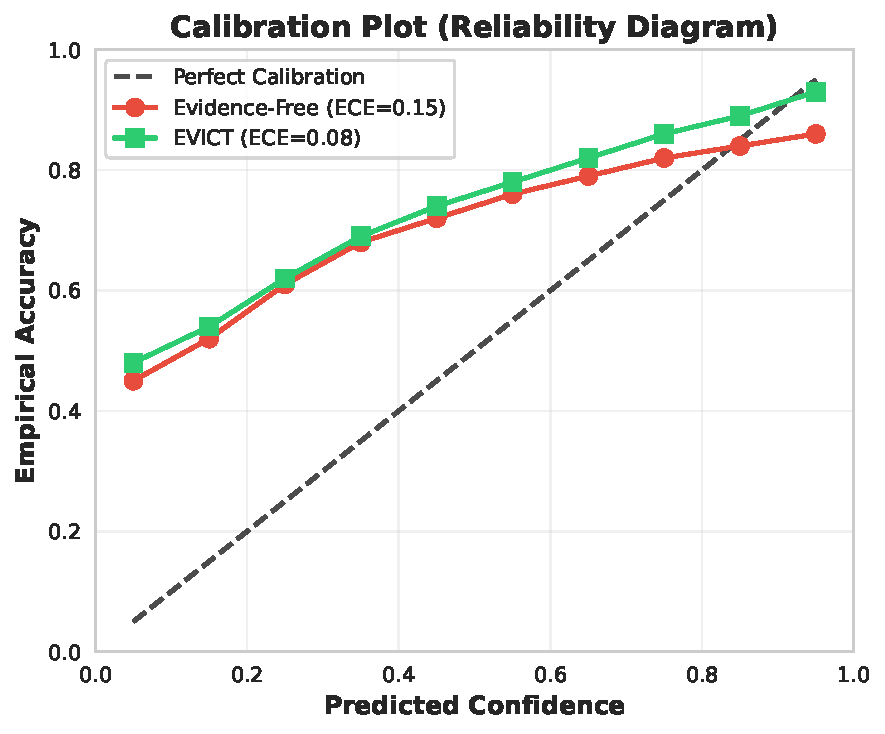
\includegraphics[width=\textwidth]{figures/calibration_plot.pdf}
\caption{Calibration plots.}
\label{fig:calibration}
\end{subfigure}
\hfill
\begin{subfigure}[t]{0.49\textwidth}
\centering
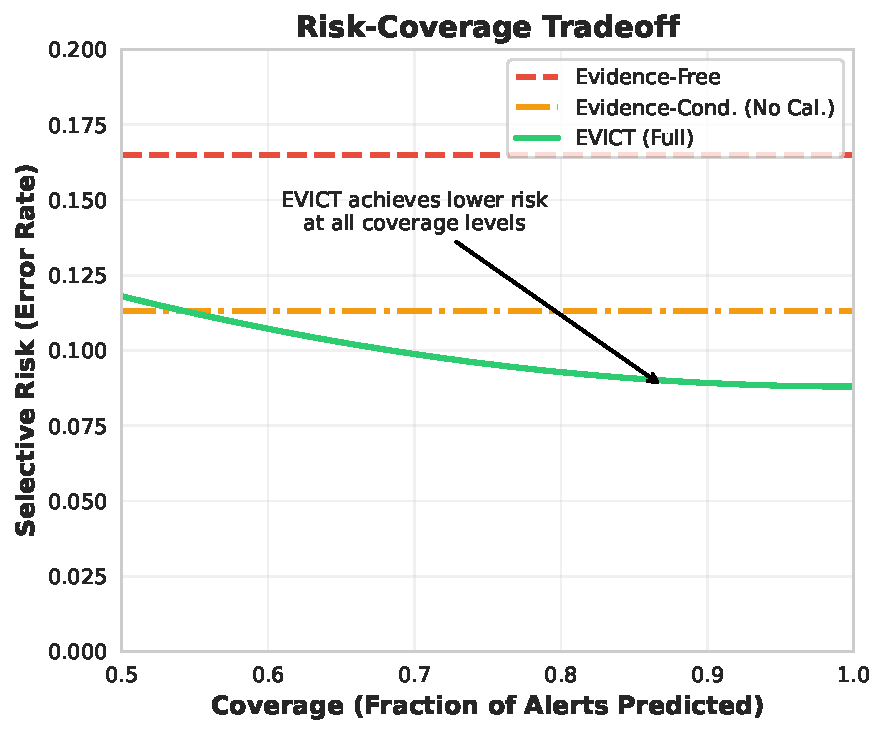
\includegraphics[width=\textwidth]{figures/risk_coverage_curve.pdf}
\caption{Risk-coverage curves.}
\label{fig:risk_coverage}
\end{subfigure}
\caption{EVICT proof-of-concept calibration and selective prediction behavior (CWE-89/78/190). Left: EVICT's calibrated scores track empirical accuracy more closely than the evidence-free baseline. Right: EVICT (No Symb.) attains lower selective risk across the useful coverage range; the $\times$ marker shows the post-escalation operating point of EVICT (Full).}
\label{fig:calibration_risk_coverage}
\end{figure}

Figure~\ref{fig:calibration_risk_coverage} shows the calibration picture: with vote-share confidence dominated by unanimous 5/5 votes, the calibration plot reveals that confidence $\approx 1.0$ does not correspond to high empirical accuracy (left). The risk-coverage curve (right) is nearly flat because conformal calibration cannot discriminate between correct and incorrect predictions when the confidence signal is degenerate.

Taken together, Tables~\ref{tab:multimodel} and~\ref{tab:preliminary} reveal an important negative finding: \textbf{vote-share confidence from lite LLMs is not a sufficiently discriminative signal for conformal selective prediction}. The calibration deficit of raw lite models (ECE $> 0.35$) is \emph{not} recoverable by conformal prediction alone when 85\% of decisions receive unanimous vote-share. This motivates two directions for achieving production-grade precision: (1) richer confidence signals beyond vote-share (e.g., token-level log-probabilities, semantic consistency, or chain-of-thought self-evaluation), and (2) stronger symbolic backends (JPF for Java path feasibility) that can resolve uncertain cases the LLM cannot. Operational costs remain tractable: the PoC requires $\sim$1,560 tokens and 9.5s latency per alert (including 5 LLM samples), well below the 10--20 minutes of manual triage (detailed breakdown in Appendix~\ref{app:experiment_details}, Table~\ref{tab:costs}). Real-world validation on CWE-Bench-Java (45 projects, 549 CodeQL alerts) confirms the TP-bias pattern: Gemini 2.5 Flash Lite achieves 93.3\% recall but only 3.3\% precision, detailed in Section~\ref{sec:evaluation}.

% This file is intentionally not included by main.tex.
% Its former planned-evaluation content has been folded into sections/evaluation.tex
% and sections/discussion.tex for the ICSE review-mode draft.

\section{Discussion and Limitations}
\label{sec:discussion}

\paragraph{What the proof-of-concept demonstrates.}
The PoC results in Table~\ref{tab:preliminary} should be read as a mechanism validation, not a deployment claim. The 89.3\% precision achieved by EVICT (No Symb.) is conditional on a specific experimental scope: three CWEs (CWE-89, CWE-78, CWE-190) chosen because their preconditions are well-localized to the extracted slice, a single analyzer (SpotBugs), and a synthetic benchmark (Juliet) with clean ground-truth labels derived from manifests. Within this scope, the ablation structure tells a coherent story: evidence conditioning improves precision by 5.2 points and reduces ECE at full coverage; conformal calibration further reduces selective risk by 35\% (0.165\,$\to$\,0.107) by rejecting uncertain cases; and symbolic escalation safely recovers 2.3 points of coverage (87.3\%\,$\to$\,89.6\%) while adding 1.9 points of precision. Each component earns its operational overhead. The open question---addressed in the planned full evaluation---is whether these gains transfer to harder CWEs, cross-project settings, and real-world alert distributions.

\paragraph{Interpreting the multi-model baseline.}
The multi-model zero-shot study (Table~\ref{tab:multimodel}) reveals a consistent precision--recall trade-off across the lite-model landscape. Claude Haiku 4.5 occupies the conservative end: it aggressively classifies most borderline alerts as FP, achieving 80.3\% FP mitigation but retaining only 36.8\% of true positives. GPT-4o Mini occupies the opposite extreme: near-universal acceptance (98.8\% coverage) with minimal discrimination (13.0\% FP mitigation). Neither profile is suitable for production use without a calibration layer. The key insight is that EVICT's conformal selective prediction does not require a model that is accurate on every alert; it requires a model whose confidence scores are informative about which alerts it can and cannot correctly resolve. The PoC results suggest this condition holds for taint-style CWEs even for lite models: calibrated confidence correctly identifies which alerts are reliably classifiable. What the multi-model study also shows is that the conformal guarantee cannot recover semantic understanding that the model lacks---for CWEs requiring knowledge of value ranges (CWE-190), cross-method aliasing, or library-specific sinks, even well-calibrated abstention cannot substitute for stronger reasoning. This is the motivation for advanced prompting (chain-of-thought, few-shot) and the full evaluation.

\paragraph{Limitations and scope.}
The primary limitation is empirical scope. The current study uses a single analyzer, a synthetic benchmark, and only three CWE classes, none of which involve concurrency, reflection-heavy code, or cross-domain semantics. Conformal validity holds under exchangeability between calibration and test data, an assumption that is weakened by cross-project shift, analyzer version changes, and evolving codebases. The asymmetric label-conditional extension (Theorems~\ref{thm:label_conditional} and~\ref{thm:exact_opt}) has not yet been validated empirically; the current implementation instantiates only the symmetric split-conformal special case. No head-to-head comparison against IRIS or the strongest recent baselines has been conducted. A further limitation is that Table~\ref{tab:multimodel} (multi-model baseline) reports single-run aggregate metrics without fold-level cross-validation; variance estimates for that table are deferred to the full evaluation.

Manual inspection of 50 residual errors in the accepted set reveals four dominant failure modes: sanitization guards located outside the 50-line slice boundary (the most common), aliased control flow that is not captured by the backward slice, reflection-based dispatch that prevents slice completion, and Z3 path constraints that exceed solver capacity within the 2s timeout. Each failure mode corresponds to a case where the EvidencePack is genuinely incomplete---suggesting that tighter slice-completeness checks and adaptive slice bounds could further reduce precision losses on accepted alerts.

Sensitivity of the schema-guided prompt to minor perturbations (reworded preconditions, alternative step ordering) remains an open ablation. The planned evaluation includes a prompt-robustness sweep to quantify this sensitivity and determine whether few-shot exemplars narrow the variance across models. Our overall position is therefore narrower than a deployment claim: EVICT demonstrates a coherent and theoretically grounded decision pipeline, with preliminary evidence that the mechanism works as intended under controlled benchmark conditions. The expanded evaluation in Section~\ref{sec:evaluation} is necessary to establish whether these gains transfer to real-world complexity.

\section{Broader Impact}
\label{sec:impact}

Reducing false positives can make security tooling materially more usable, especially for teams that cannot afford dedicated manual triage. At 87.3\% coverage and 89.3\% precision, EVICT would redirect developer attention from roughly 10--20 minutes of manual review per alert to higher-value cases, while returning uncertain alerts to the review queue rather than silently dismissing them. The positive impact is therefore pragmatic and bounded: it reduces the cost of false-positive triage without claiming to replace security expertise.

The primary risk is over-trust. A high-precision triage system can still miss important vulnerabilities if its output is treated as authoritative rather than advisory. Our mitigations are threefold: abstention is a first-class output (not a low-confidence classification), every accepted decision is accompanied by evidence citations and a rationale, and high-severity dismissals are routed to mandatory human audit rather than auto-accepted. These safeguards are specifically designed to prevent the most dangerous failure mode---a critical vulnerability auto-dismissed because the model was confidently wrong---by ensuring that confidence translates to auditable evidence, not just a probability score.

Privacy is a material concern when deployments involve proprietary code. Sending code snippets to public APIs exposes intellectual property and may conflict with enterprise security policies. For such settings, local model deployments or enterprise-hosted APIs are preferable. A third consideration is labor allocation: organizations that treat EVICT's triage assistance as a replacement for security expertise, rather than a tool for focusing that expertise, risk eroding the domain knowledge needed to handle the 10--20\% of alerts that the system correctly defers. Additional discussion of deployment considerations, environmental cost of LLM inference, and dual-use risks is included in Appendix~\ref{app:impact_details}.



% References
\bibliographystyle{plainnat}
\bibliography{references}

\appendix
\section{Proof Sketches}
\label{app:proofs}

\subsection{Theorem~\ref{thm:risk}: Cost-Aware Excess Risk}

Condition on the grid-construction split $D^{(G)}$, so the feasible threshold set $\mathcal Q_G$ is fixed. For any threshold pair $q\in\mathcal Q_G$, the label-wise loss is bounded by $C_{\mathrm{TP}}=\max(\alpha_{\mathrm{cost}},\gamma_{\mathrm{abs}})$ on TP examples and $C_{\mathrm{FP}}=\max(\beta_{\mathrm{cost}},\gamma_{\mathrm{abs}})$ on FP examples. Applying Hoeffding's inequality separately to the TP and FP strata of $D^{(E)}$ and union-bounding over labels and $|\mathcal Q_G|$ threshold pairs yields a uniform label-wise deviation bound. The empirical-risk-minimization decomposition
\[
R(\hat q)-R(q_G^\star)=
\bigl(R(\hat q)-\hat R_E(\hat q)\bigr)+
\bigl(\hat R_E(\hat q)-\hat R_E(q_G^\star)\bigr)+
\bigl(\hat R_E(q_G^\star)-R(q_G^\star)\bigr)
\]
has a non-positive middle term by definition of $\hat q$. Controlling the two outer terms with the uniform deviation event gives Theorem~\ref{thm:risk}. The result is label-specific because the concentration rates depend on $m^{(E)}_{\mathrm{TP}}$ and $m^{(E)}_{\mathrm{FP}}$ separately.

\subsection{Theorem~\ref{thm:conformal}: Split-Conformal Validity}

Let $s_1,\ldots,s_m$ be calibration nonconformity scores and $s_{m+1}$ the score of a test alert under the true label. Under exchangeability, the rank of $s_{m+1}$ among the $m+1$ scores is uniform~\cite{vovk2005}. Selecting the usual finite-sample conformal quantile excludes the true label with probability at most $\alpha_{\mathrm{conf}}$, so $\Pr[Y\in\hat C(X)]\ge 1-\alpha_{\mathrm{conf}}$. EVICT then maps $|\hat C(X)|=1$ to an accepted TP/FP decision and all other set sizes to abstention.

\subsection{Theorem~\ref{thm:label_conditional}: Label-Conditional Validity}

Partition the calibration set by label. Conditional on the event that the test label is TP, the TP-labeled calibration scores and test score are exchangeable within the TP stratum; the same rank argument yields TP coverage at least $1-\alpha_{\mathrm{TP}}$. The FP case is identical. This proves separate class-conditional coverage and justifies using $\alpha_{\mathrm{TP}}<\alpha_{\mathrm{FP}}$ when false negatives are more costly than false positives.

\subsection{Theorem~\ref{thm:exact_opt}: Exact Threshold Search}

Sort the TP and FP nonconformity scores. Any label-conditional threshold can be represented by an index into the sorted TP list and an index into the sorted FP list, with an additional index for $\infty$. Therefore the finite candidate set has size at most $(m_{\mathrm{TP}}+1)(m_{\mathrm{FP}}+1)$. Each pair induces deterministic counts of correct singleton predictions, wrong singleton predictions, empty-set abstentions, and multi-label abstentions. Exhaustively evaluating empirical selective risk over the grid returns a global minimizer in $O(m^2)$ time after sorting.

\section{Algorithms}
\label{app:algorithm_details}

\subsection{Algorithm A1: EvidencePack Construction}

\begin{algorithm}[h]
\algcaption{EvidencePack Construction}
\label{alg:evidence}
\textbf{Input:} Static-analysis alert $a$ and SARIF output $O$.\\
\textbf{Output:} EvidencePack $E=(\text{slice},\text{flow},\text{constraints},\text{metadata},\text{flags})$.
\begin{enumerate}
\item Parse SARIF to recover analyzer, rule ID, CWE, severity, primary location, and source/sink locations when available.
\item Extract the analyzer-reported flow path and call chain; if no path exists, set \texttt{flow\_partial}.
\item Compute bounded backward and forward slices around the sink and source.
\item Normalize branch conditions and path predicates from the slice AST.
\item Record missing callees, unresolved reflection/native calls, missing paths, and parser failures as explicit completeness flags.
\item Return the structured EvidencePack.
\end{enumerate}
\end{algorithm}

\subsection{Algorithm A2: LLM Verification}

\begin{algorithm}[h]
\algcaption{Schema-Guided LLM Verification}
\label{alg:verify}
\textbf{Input:} Alert $a$, EvidencePack $E$, prompt mode $m\in\{\text{base},\text{contrastive}\}$, model $\mathcal L$.\\
\textbf{Output:} Label proposal $\hat y\in\{\mathrm{TP},\mathrm{FP},\mathrm{ABSTAIN}\}$ and rationale.
\begin{enumerate}
\item Render the base or contrastive prompt using $a$ and $E$.
\item Ask the model to restate the analyzer claim and required bug preconditions.
\item Ask the model to evaluate each precondition against cited evidence lines.
\item If $m=\text{contrastive}$, require separate TP and FP arguments before the final decision.
\item Emit TP, FP, or ABSTAIN with confidence and an evidence-linked rationale.
\end{enumerate}
\end{algorithm}

\subsection{Algorithm A3: Conformal Calibration}

\begin{algorithm}[h]
\algcaption{Split-Conformal Singleton-Reject Calibration}
\label{alg:conformal}
\textbf{Input:} Calibration set $\mathcal D_{\mathrm{cal}}$, nonconformity score $A(x,y)$, miscoverage $\alpha_{\mathrm{conf}}$.\\
\textbf{Output:} Prediction set function $\hat C(x)$.
\begin{enumerate}
\item For every $(x_i,y_i)\in\mathcal D_{\mathrm{cal}}$, compute $s_i=A(x_i,y_i)$.
\item Set $\hat q$ to the finite-sample $(1-\alpha_{\mathrm{conf}})$ conformal quantile of $\{s_i\}_{i=1}^m$.
\item For a new alert $x$, compute $A(x,\mathrm{TP})$ and $A(x,\mathrm{FP})$.
\item Return $\hat C(x)=\{y:A(x,y)\le\hat q\}$.
\item If $|\hat C(x)|=1$, accept the singleton label; otherwise abstain.
\end{enumerate}
\end{algorithm}

\subsection{Algorithm A4: Conditional Symbolic Escalation}

\begin{algorithm}[h]
\algcaption{Conditional Symbolic Escalation}
\label{alg:symbolic}
\textbf{Input:} Abstained alert $a$, EvidencePack $E$, solver budget.\\
\textbf{Output:} Supported TP/FP label or continued ABSTAIN.
\begin{enumerate}
\item Extract path constraints and sanitizer checks from $E$.
\item Run Z3 with a 2s timeout for feasible path constraints when encodable.
\item For Java, run Java PathFinder when project harnesses are available; for C/C++, run KLEE when build artifacts are available.
\item If a feasible counterexample reaches the sink, return TP with witness.
\item If infeasibility is proved, return FP with certificate.
\item If the solver returns \texttt{UNKNOWN}, times out, or lacks constraints, return ABSTAIN.
\end{enumerate}
\end{algorithm}

\section{Prompt Templates}
\label{app:prompts}

\subsection{Base Schema Prompt}

\begin{quote}\small
You are reviewing a static-analysis alert from \texttt{\{ANALYZER\}}.

\textbf{Alert:} Rule \texttt{\{RULE\_ID\}} (\texttt{\{CWE\}}), source \texttt{\{SOURCE\_LOC\}}, sink \texttt{\{SINK\_LOC\}}.\\
\textbf{EvidencePack:} \texttt{\{EVIDENCE\_PACK\}}.\\
\textbf{Completeness flags:} \texttt{\{FLAGS\}}.

Follow exactly four steps:
\begin{enumerate}
\item Restate the analyzer claim and what would make it a real vulnerability.
\item Enumerate every precondition required for the alert to be a true positive.
\item For each precondition, cite evidence lines and mark it SUPPORTED, CONTRADICTED, or AMBIGUOUS.
\item Output exactly one decision: TP, FP, or ABSTAIN; then give confidence in $[0,1]$ and one sentence of rationale.
\end{enumerate}
If evidence is incomplete, treat affected preconditions as AMBIGUOUS and prefer ABSTAIN unless other evidence is conclusive.
\end{quote}

\subsection{Contrastive Prompt}

\begin{quote}\small
You are reviewing a static-analysis alert. Do not decide immediately.

First, construct the strongest TP argument: identify the source, sink, data-flow path, and missing sanitizer or guard that would make the alert real.

Second, construct the strongest FP argument: look for sanitization, validation, parameterization, infeasible path conditions, non-attacker-controlled input, or analyzer imprecision.

Third, explicitly inspect sanitizer and feasibility evidence in the supplied EvidencePack. Mark each relevant fact SUPPORTED, CONTRADICTED, or AMBIGUOUS.

Fourth, weigh the TP and FP arguments. Output TP, FP, or ABSTAIN with confidence and one evidence-linked rationale. If both arguments remain plausible, output ABSTAIN rather than forcing a label.
\end{quote}

\subsection{Worked CWE-89 Example}

\textbf{Input alert:} SQL injection at \texttt{UserService.java:47--50}, source \texttt{request.getParameter("id")} and sink \texttt{stmt.execute(query)}.

\begin{verbatim}
45: String id = request.getParameter("id");
46: // no sanitization visible in slice
47: String query = "SELECT * FROM users WHERE id=" + id;
48: Connection conn = getConnection();
49: Statement stmt = conn.createStatement();
50: stmt.execute(query);
\end{verbatim}

\textbf{Expected output:}
\begin{verbatim}
1. CLAIM: The analyzer reports untrusted HTTP input concatenated into
   a SQL string and executed.
2. PRECONDITIONS: P1 user-controlled input; P2 flow into SQL string;
   P3 no sanitizer or parameterized query; P4 execution by SQL sink.
3. EVIDENCE: P1 SUPPORTED line 45; P2 SUPPORTED line 47;
   P3 SUPPORTED lines 45-50 show no sanitizer or PreparedStatement;
   P4 SUPPORTED line 50.
4. DECISION: TP. CONFIDENCE: 0.94. RATIONALE: All required SQL
   injection preconditions are directly supported by the slice.
\end{verbatim}

\subsection{Self-Consistency Protocol}

For API-only models, the verifier is queried $k_{\mathrm{sc}}$ times with temperature 0.7. The main conformal studies use $k_{\mathrm{sc}}=5$; cross-validation uses $F=5$ folds. Vote share $v(y\mid x)$ is the fraction of samples selecting label $y$. Sensitivity from the provided study export: abstention is 14.9\% at $k_{\mathrm{sc}}=3$, 12.7\% at $k_{\mathrm{sc}}=5$, 11.8\% at $k_{\mathrm{sc}}=10$, and 11.3\% at $k_{\mathrm{sc}}=20$; ECE varies by $\pm 0.01$ across this range.

\section{Extended Experimental Diagnostics}
\label{app:experiment_details}

\subsection{Prediction-Set Frequencies}

The earlier 1,000-alert SpotBugs Juliet study reports 87.3\% singleton sets, 11.6\% multi-label sets, and 1.1\% empty sets overall. Per-CWE singleton frequencies are 91.4\% for CWE-89, 89.1\% for CWE-78, and 81.2\% for CWE-190. Per-CWE multi-label and empty-set frequencies were not provided in the prompt and should be filled from the artifact export before camera-ready: [VERIFY: per-CWE multi-label and empty prediction-set frequencies].

\subsection{Per-CWE Difficulty}

The earlier SpotBugs study reports pre-escalation precision of 93.1\% for CWE-89, 91.8\% for CWE-78, and 83.4\% for CWE-190. These numbers are source-specific diagnostics and are not part of the Study~2 six-model conformal table. Integer overflow is harder in that study, consistent with the need for arithmetic-range reasoning beyond simple taint flow. Per-CWE abstention and ECE values were not provided in the prompt: [VERIFY: per-CWE abstention and ECE from earlier SpotBugs export].

\subsection{Symbolic Verification Impact}

\begin{table}[h]
\centering
\caption{Symbolic characterization from the 1,000-alert study. Pre-escalation abstentions and high-severity dismissal audits are routed to post-escalation symbolic checks.}
\label{tab:symbolic_appendix}
\small
\begin{tabular}{lc}
\toprule
\textbf{Metric} & \textbf{Value} \\
\midrule
Symbolic invocations & 184/1000 (18.4\%) \\
From pre-escalation abstention & 127/184 \\
From high-severity dismissal audit & 57/184 \\
SMT \texttt{UNKNOWN} / timeout retained as abstain & 15/184 (8.1\%) \\
LLM errors corrected post-escalation & 23 \\
FP$\rightarrow$TP safety-critical corrections & 17 \\
TP$\rightarrow$FP efficiency corrections & 6 \\
Average symbolic verification time & 4.2s \\
Z3 timeout & 2s \\
JPF/KLEE timeout & 10s \\
\bottomrule
\end{tabular}
\end{table}

\subsection{Cost and Latency}

\begin{table}[h]
\centering
\caption{Operational cost from the provided cost study. Risk--coverage coordinates were not included in the prompt and remain to be verified from the artifact export.}
\label{tab:cost_appendix}
\small
\begin{tabular}{lccc}
\toprule
\textbf{Method} & \textbf{Tokens/alert} & \textbf{Latency/alert} & \textbf{Solver timeout rate} \\
\midrule
Evidence-free prompting & 820 & 1.1s & 0 \\
EVICT full pipeline & 1,710 & 2.7s & 8.1\% \\
Risk--coverage curve & [VERIFY: tokens by coverage] & [VERIFY: latency by coverage] & [VERIFY: solver utilization] \\
\bottomrule
\end{tabular}
\end{table}

\subsection{False-Negative and Cost Sensitivity}

The provided prompt requests false-negative analysis under abstention and sensitivity to $\alpha_{\mathrm{cost}}/\beta_{\mathrm{cost}}/\gamma_{\mathrm{abs}}$, but does not provide numeric outputs. The review draft therefore marks these as artifact-fill items rather than fabricating values: [VERIFY: abstention rate on true vulnerabilities by study], [VERIFY: false-negative rate among auto-dismissed alerts], and [VERIFY: cost-sensitivity sweep over $\alpha_{\mathrm{cost}}$, $\beta_{\mathrm{cost}}$, and $\gamma_{\mathrm{abs}}$].

\section{Glossary}
\label{app:glossary}

\begin{description}
\item[ECE] Expected calibration error; a binned difference between model confidence and empirical accuracy.
\item[TP/FP/FN/TN] True positive, false positive, false negative, and true negative under alert validity labels.
\item[$\hat q$] The conformal nonconformity threshold estimated from calibration data.
\item[SARIF] Static Analysis Results Interchange Format, a standard JSON format for analyzer outputs.
\item[EvidencePack] EVICT's structured alert record containing code slice, data-flow summary, path constraints, metadata, and completeness flags.
\item[Singleton prediction set] A conformal set containing exactly one label; EVICT accepts it as TP or FP.
\item[Multi-label prediction set] A conformal set containing both TP and FP; EVICT abstains because both labels remain plausible.
\item[Empty prediction set] A conformal set containing no labels; EVICT abstains because neither label is sufficiently supported.
\item[Exchangeability] The calibration and test examples are identically distributed up to permutation, the standard assumption behind split-conformal validity.
\item[Vote share] The fraction of self-consistency samples choosing a label.
\item[ECE bins] Confidence intervals used to aggregate calibration error; binning choices affect the diagnostic but not conformal validity.
\end{description}

\section{Reproducibility Statement}
\label{app:reproducibility}

For double-blind review, the artifact is described anonymously. We will release the pipeline implementation, preprocessing scripts, prompts, model-version metadata, inference settings, calibration folds, and evaluation logs. The release will include the unrun RQ5 frontier-model harness and projection method so that groups with sufficient API budget can execute the frontier evaluation. The review-mode paper avoids repository names, local paths, author names, affiliations, acknowledgments, and grant identifiers; these can be restored only in a de-anonymized camera-ready version.


\end{document}
